% Chapter Template

\chapter{Introduction} % Main chapter title

\label{Chapter1} % Change X to a consecutive number; for referencing this chapter elsewhere, use \ref{ChapterX}

%----------------------------------------------------------------------------------------
%	SECTION 1
%----------------------------------------------------------------------------------------

\section{Imaging}
Intensity \cite{physicsGhost}

%-----------------------------------
%	SUBSECTION 1
%-----------------------------------
\section{Two-Photon Imaging}

\subsection{Two-Photon Imaging using entangled photon pairs}
A two-photon optical imaging experiment was perfomed based on the quantum nature of the \textit{signal} and \textit{idler}
photons pairs produced in spontaneous parametric down-conversion\cite{pittman}.
\begin{figure}[h]
\centering
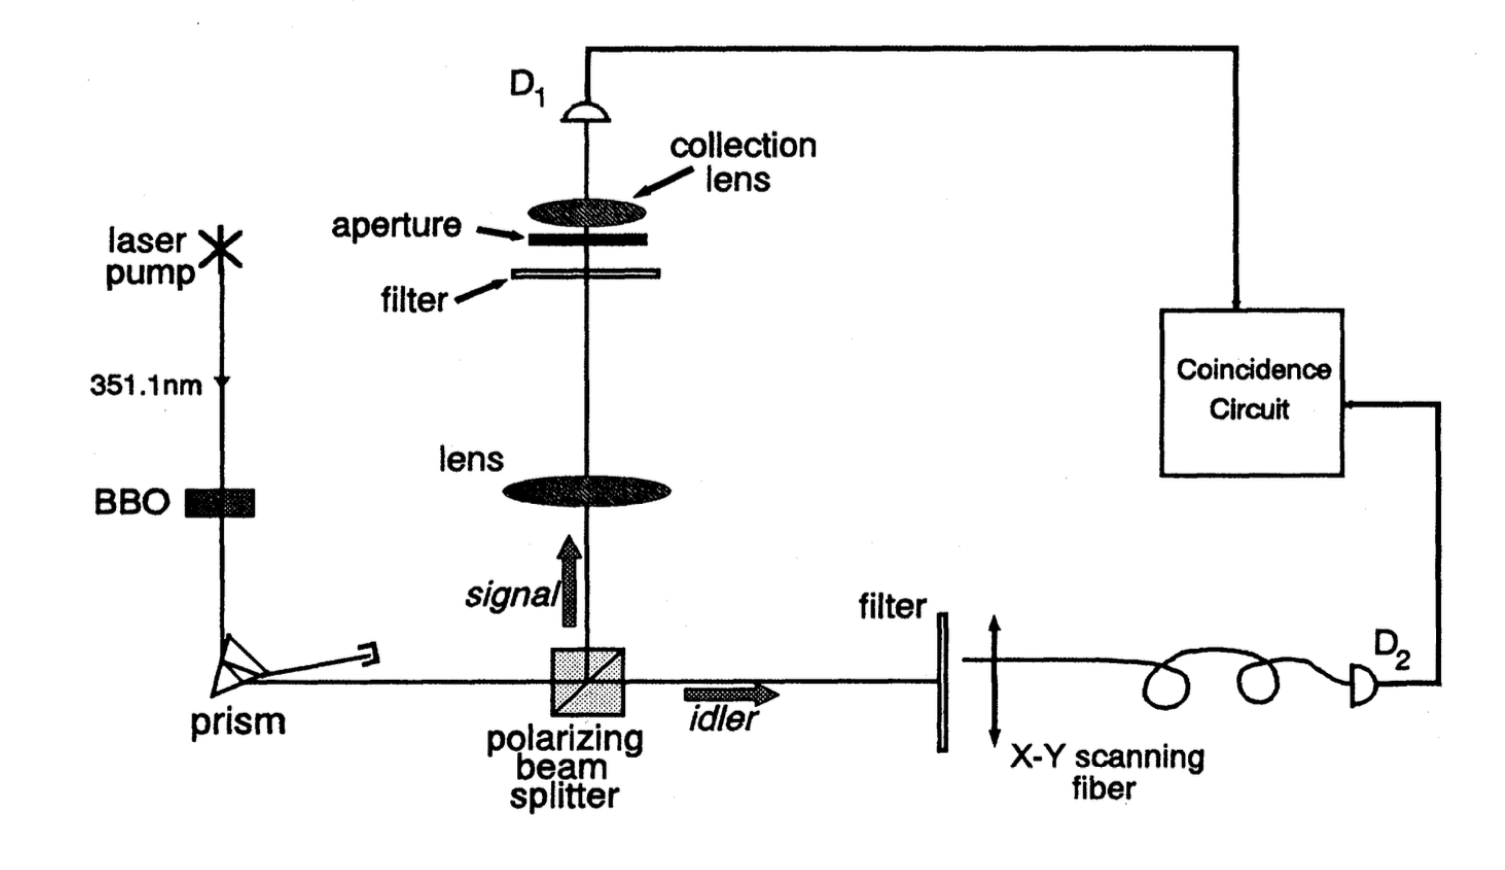
\includegraphics[width=0.5\textwidth]{Figures/pittman.png}
\caption{Cartoon schematic of the experimental setup used by Pittman, Taken from \cite{pittman}} 
\label{fig:pittman}
\end{figure}
An important fact of this experiment is the use of a lens in the signal beam that establishes an image plane with the definitive point-by-point correspondence object(mask) plane.




\subsection{Two-photon Imaging Using Thermal Sources}

In \cite{thermal} they compared ghost Imaging using entanglement versus Classical correlated light. read and information in \cite{thermalAlejandra}. here i talk about coherence and intensity fluctuations \cite{intensity}

\subsection{Simulations}

No\cite{simulated}
%----------------------------------------------------------------------------------------
%	SECTION 2
%----------------------------------------------------------------------------------------



